\batchmode
\makeatletter
\def\input@path{{/Users/samharper/Dropbox/work/research/projects/FARS/mvc-bayes/work/talk/}}
\makeatother
\documentclass[english]{beamer}\usepackage[]{graphicx}\usepackage[]{color}
% maxwidth is the original width if it is less than linewidth
% otherwise use linewidth (to make sure the graphics do not exceed the margin)
\makeatletter
\def\maxwidth{ %
  \ifdim\Gin@nat@width>\linewidth
    \linewidth
  \else
    \Gin@nat@width
  \fi
}
\makeatother

\definecolor{fgcolor}{rgb}{0.345, 0.345, 0.345}
\newcommand{\hlnum}[1]{\textcolor[rgb]{0.686,0.059,0.569}{#1}}%
\newcommand{\hlstr}[1]{\textcolor[rgb]{0.192,0.494,0.8}{#1}}%
\newcommand{\hlcom}[1]{\textcolor[rgb]{0.678,0.584,0.686}{\textit{#1}}}%
\newcommand{\hlopt}[1]{\textcolor[rgb]{0,0,0}{#1}}%
\newcommand{\hlstd}[1]{\textcolor[rgb]{0.345,0.345,0.345}{#1}}%
\newcommand{\hlkwa}[1]{\textcolor[rgb]{0.161,0.373,0.58}{\textbf{#1}}}%
\newcommand{\hlkwb}[1]{\textcolor[rgb]{0.69,0.353,0.396}{#1}}%
\newcommand{\hlkwc}[1]{\textcolor[rgb]{0.333,0.667,0.333}{#1}}%
\newcommand{\hlkwd}[1]{\textcolor[rgb]{0.737,0.353,0.396}{\textbf{#1}}}%
\let\hlipl\hlkwb

\usepackage{framed}
\makeatletter
\newenvironment{kframe}{%
 \def\at@end@of@kframe{}%
 \ifinner\ifhmode%
  \def\at@end@of@kframe{\end{minipage}}%
  \begin{minipage}{\columnwidth}%
 \fi\fi%
 \def\FrameCommand##1{\hskip\@totalleftmargin \hskip-\fboxsep
 \colorbox{shadecolor}{##1}\hskip-\fboxsep
     % There is no \\@totalrightmargin, so:
     \hskip-\linewidth \hskip-\@totalleftmargin \hskip\columnwidth}%
 \MakeFramed {\advance\hsize-\width
   \@totalleftmargin\z@ \linewidth\hsize
   \@setminipage}}%
 {\par\unskip\endMakeFramed%
 \at@end@of@kframe}
\makeatother

\definecolor{shadecolor}{rgb}{.97, .97, .97}
\definecolor{messagecolor}{rgb}{0, 0, 0}
\definecolor{warningcolor}{rgb}{1, 0, 1}
\definecolor{errorcolor}{rgb}{1, 0, 0}
\newenvironment{knitrout}{}{} % an empty environment to be redefined in TeX

\usepackage{alltt}
\usepackage[T1]{fontenc}
\usepackage[latin9]{inputenc}
\setcounter{secnumdepth}{3}
\setcounter{tocdepth}{3}
\usepackage{amsbsy}
\usepackage{amstext}
\usepackage{amssymb}
\usepackage{graphicx}

\makeatletter

%%%%%%%%%%%%%%%%%%%%%%%%%%%%%% LyX specific LaTeX commands.
%% Because html converters don't know tabularnewline
\providecommand{\tabularnewline}{\\}

%%%%%%%%%%%%%%%%%%%%%%%%%%%%%% Textclass specific LaTeX commands.
 % this default might be overridden by plain title style
 \newcommand\makebeamertitle{\frame{\maketitle}}%
 % (ERT) argument for the TOC
 \AtBeginDocument{%
   \let\origtableofcontents=\tableofcontents
   \def\tableofcontents{\@ifnextchar[{\origtableofcontents}{\gobbletableofcontents}}
   \def\gobbletableofcontents#1{\origtableofcontents}
 }

%%%%%%%%%%%%%%%%%%%%%%%%%%%%%% User specified LaTeX commands.
\usepackage{etex}

\usetheme{Madrid}
%\usecolortheme{beaver}

%gets rid of bottom navigation bars
\setbeamertemplate{footline}[frame number]{}

%gets rid of navigation symbols
\setbeamertemplate{navigation symbols}{}

\usepackage[onecol]{hackthefootline}
\htfconfig{title=none, authinst=none, date=short}

\setbeamertemplate{footline}{bg=white}

% \setbeamercovered{transparent}
% or whatever (possibly just delete it)

\AtBeginSection[]{
  \begin{frame}
  \vfill
  \centering
  \begin{beamercolorbox}[sep=8pt,center,shadow=true,rounded=true]{title}
    \usebeamerfont{title}\insertsectionhead\par%
  \end{beamercolorbox}
  \vfill
  \end{frame}
}

\renewcommand\footnotesize{\fontsize{7}{7} \selectfont}

\renewcommand{\thefootnote}{}
% for unnumbered footnotes

\usepackage{hyperref}
\hypersetup{
  colorlinks,
  citecolor=violet,
  linkcolor=white,
  urlcolor=blue}

% for arrows
\usepackage{tikz}
\usepackage{pgfplots}
\usepackage{verbatim}
\usetikzlibrary{arrows,shapes,backgrounds}
\tikzstyle{every picture}+=[remember picture]
\tikzstyle{na} = [baseline=-.5ex]
\def\checkmark{\tikz\fill[scale=0.4](0,.35) -- (.25,0) -- (1,.7) -- (.25,.15) -- cycle;} 

% for code
\usepackage{listings}

%Macros to make graphics insertions easy
%Command for sizing to width    \figw{file}{fraction of \textwidth}
\newcommand{\figw}[2]{\centerline{\includegraphics[width=#2\textwidth]{#1}}}
%Command for sizing to height   \figh{file}{fraction of \textheight}
\newcommand{\figh}[2]{\centerline{\includegraphics[height=#2\textheight]{#1}}}
%Use \figh{graphics file name}{1} to size to whole text height
%For graphics needing no shrinkage:  \fig{file}
\newcommand{\fig}[1]{\centerline{\includegraphics{#1}}}

% For making stata journal type tables
%\usepackage{stata}

% conditional independence
\newcommand{\Perp}{\perp\!\!\!\perp}
\usepackage{fancybox}

\makeatother

\usepackage{babel}
\IfFileExists{upquote.sty}{\usepackage{upquote}}{}
\begin{document}

\title[MVC-Bayes ]{Would Stronger Seat Belt Laws Reduce Motor Vehicle Crash Deaths?}

\subtitle{Semi-Bayesian Analysis}

\author[S. Harper ]{Sam Harper\inst{1,2} }

\institute[McGill]{\inst{1}Epidemiology, Biostatistics \& Occupational Health, McGill
University \and\inst{2}Institute for Health and Social Policy, McGill
University}

\date[22 Oct 2018]{Erasmus Medical Center, 22 Oct 2018}
\makebeamertitle
\begin{frame}{Why Am I Here?}


\begin{columns}
    \begin{column}{0.5\textwidth}
        \begin{itemize}
            \item[] Smarter Choices involves $\rightarrow$ producing evidence about interventions.
        \end{itemize}
    \end{column}
    \begin{column}{0.5\textwidth}
        \figw{SG-AL4.png}{.9}
    \end{column}
\end{columns}


\begin{columns}
    \begin{column}{0.4\textwidth}
        \begin{itemize}
            \item[] In this talk I want to discuss how to make "smarter choices" when producing that evidence.
        \end{itemize}
    \end{column}
    \begin{column}{0.6\textwidth}
        \figw{SG-NL-perinatal.png}{1}
    \end{column}
\end{columns}
\end{frame}
%

\section{Background}
\begin{frame}[plain]{}

\footnote{{\tiny{}Source: OECD (2018), Road accidents (indicator). doi: 10.1787/2fe1b899-en
(Accessed on 21 October 2018)}}
\begin{center}
\includegraphics[width=0.9\paperwidth]{0_Users_samharper_Dropbox_work_research_projects_FARS_mvc-bayes_work_talk_oecd-mvc-trends.png}
\par\end{center}

\end{frame}
%
\begin{frame}{Context of Motor Vehicle Deaths in USA}
\begin{itemize}
\item Seat belt use reduces motor vehicle crash (MVC) deaths.\medskip{}
\item<2-> First mandatory seat belt law in 1984 (NY state).\medskip{}
\item<3-> Evidence that mandatory seat belt laws:
\begin{itemize}
\item Increase seat belt use.
\item Reduced MVC death rates.\medskip{}
\end{itemize}
\item<4-> Current laws come in two varieties:
\begin{itemize}
\item Secondary enforcement: Consequent to another violation
\item Primary enforcement: Seen not wearing seat belt
\end{itemize}
\medskip{}

\item<5-> Presently, 35 states with primary enforcement, 15 with secondary.
\end{itemize}
\end{frame}
%
\begin{frame}[plain]{}
\begin{alertblock}{Question}

Should states with secondary enforcement upgrade to primary?
\end{alertblock}
\end{frame}
%
\begin{frame}{Current laws as of 2017}
\footnote{{\tiny{}Source: Insurance Institute for Highway Safety}}
\begin{center}
\includegraphics[width=0.85\paperwidth]{1_Users_samharper_Dropbox_work_research_projects_FARS_mvc-bayes_work_talk_figA2a.png}
\par\end{center}

\end{frame}
%
\begin{frame}{}
\footnote{{\tiny{}Pew Trusts, Stateline, April 28, 2017. http://bit.ly/2pFTFPp}}
\begin{center}
\includegraphics[width=0.85\paperwidth]{2_Users_samharper_Dropbox_work_research_projects_FARS_mvc-bayes_work_talk_bergal-collated.png}
\par\end{center}

\end{frame}
%
\begin{frame}[plain]{Should Colorado upgrade to primary?}
\begin{center}
\includegraphics[width=0.9\paperwidth]{3_Users_samharper_Dropbox_work_research_projects_FARS_mvc-bayes_work_talk_co-cdot-quote.png}
\par\end{center}

\end{frame}
%
\begin{frame}{Hang on...}
\footnote{http://www.9news.com, Dec 8, 2016.}


\begin{columns}
    \begin{column}{0.6\textwidth}
        \begin{itemize}
            \item[] "CDOT should be concerned with building and maintaining our roads. Not joining the nanny crowd trying to protect us from our own bad decisions. \medskip{}
            \item[] ...Darwinism exists for a reason. If people want to meet their windshields at 60 miles and hour and remove themselves from the gene pool, that might be good for us in the long run. \medskip{}
            \item[] It's not a difficult sell to ask people to save their own lives. \textcolor{red}{But it shouldn't be done at gunpoint}."
        \end{itemize}
    \end{column}
    \begin{column}{0.4\textwidth}
        \figw{co-concerned.png}{.9}
    \end{column}
\end{columns}
\end{frame}
%
\begin{frame}{Potential unintended consequences (``Driving While Black'')}
\footnote{{\tiny{}https://www.aclu.org/report/racial-disparities-florida-safety-belt-law-enforcement}}
\begin{center}
\includegraphics[width=0.9\paperwidth]{4_Users_samharper_Dropbox_work_research_projects_FARS_mvc-bayes_work_talk_aclu-disparities.png}
\par\end{center}

\end{frame}
%
\begin{frame}{Rationale for Bayesian evaluation}
\begin{itemize}
\item Prior evidence on primary laws:
\begin{itemize}
\item Strong evidence they reduce deaths and increase seat belt use;
\item This evidence is dated (1990s, early 2000s).\medskip{}
\end{itemize}
\item 16 states have upgraded to primary since 2000.

\medskip{}

\end{itemize}
Our aims:
\begin{enumerate}
\item Evaluate recent policy changes.{*}\footnote{{*}Harper \& Strumpf, \textit{Am J Prev Med} 2017.}
\item Combine the evaluation of recent data with prior evidence.
\item Provide updated evidence on the impact of upgrading to primary enforcement.
\end{enumerate}
\end{frame}
%
\begin{frame}{Intuition for Bayesian analysis}
\begin{itemize}
\item We will generate new empirical evidence on the impact of policy changes
since 2000.
\item How should we approach inference from this study?\medskip{}
\end{itemize}

\pause{}
\begin{itemize}
\item Frequentist analysis assumes \textbf{zero} background information.
\item Equivalent to belief that primary laws just as likely to:
\begin{itemize}
\item Decrease death rates by a factor of 100 or 10\textit{;}
\item \textit{Increase} death rates by a factor 10 or 100.
\end{itemize}
\medskip{}

\end{itemize}

\pause{}
\begin{itemize}
\item Bayesian inference explicitly incorporates prior information to estimate
the posterior probability distribution:
\end{itemize}
\[
\underbrace{P(\theta|D)}_{\textrm{posterior probability}}\propto\underbrace{P(D|\theta)}_{\textrm{ likelihood }}\times\underbrace{P(\theta)}_{\textrm{prior probability}}
\]

\end{frame}
%
\begin{frame}{Prior empirical evidence on upgrades to primary enforcement}
\begin{itemize}
\item 3 high-quality studies on MVC death rates:\footnote{Estimates from random effects meta-analysis.}
\item Mean estimate: -0.5 deaths/billion VMT (-0.7, -0.3)\textcolor{red}{$\rightsquigarrow$1500
deaths/yr.}
\item Prediction interval for new trial: (-1.97, 0.94).\textcolor{red}{$\rightsquigarrow$(-6000,
+3000).}
\item On relative scale $RR=0.95$, $95\%CI=0.83,1.09$
\end{itemize}
\begin{center}
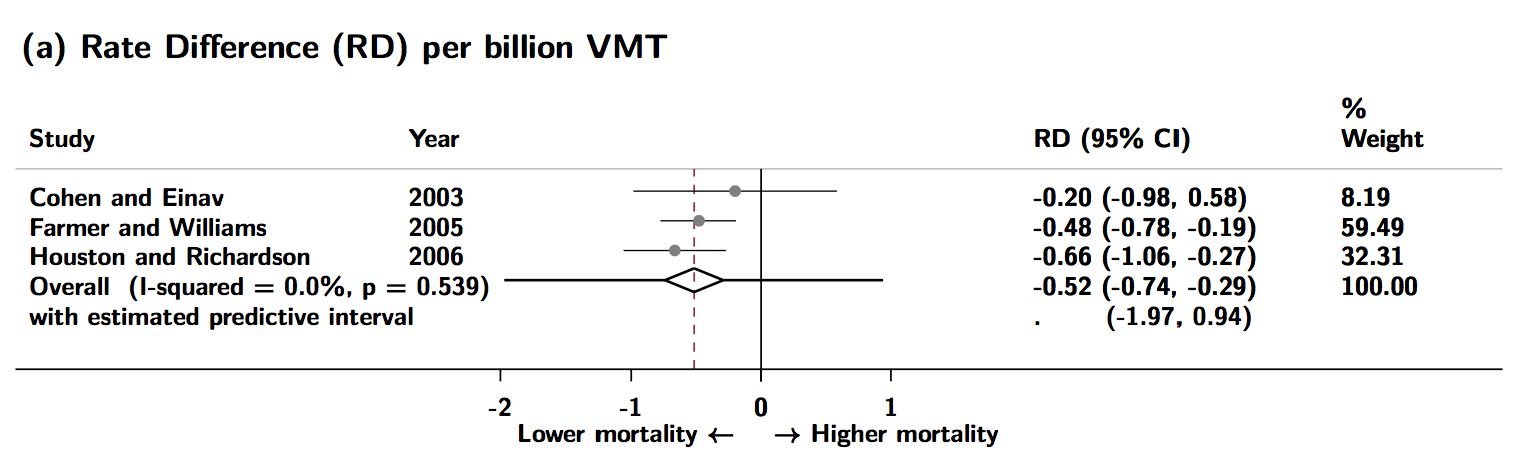
\includegraphics[width=0.95\paperwidth,bb = 0 0 200 100, draft, type=eps]{/Users/samharper/Dropbox/FARS/mvc-bayes/work/talk/meta-mvc.png}
\par\end{center}

\end{frame}
%
\begin{frame}{Prior empirical evidence on upgrades to primary enforcement}
\begin{itemize}
\item 6 moderate-quality studies on proportion belted:\footnote{Hedlund et al. (2008). Estimates from random effects meta-analysis.}
\item Average estimate: 0.13 (0.10, 0.16). \textcolor{red}{$\rightsquigarrow$13
percentage points.}
\item Prediction interval for new ``trial'': (0.03, 0.23).
\item On relative scale $RR=1.3$, $95\%CI=1.08,1.58$
\end{itemize}
\begin{center}
\includegraphics[width=0.95\paperwidth]{5_Users_samharper_Dropbox_work_research_projects_FARS_mvc-bayes_work_talk_meta-pb.png}
\par\end{center}

\end{frame}
%

\section{Methods}
\begin{frame}{Semi-Bayesian analysis via data augmentation}
\begin{itemize}
\item Data augmentation expresses prior information by adding empirical
observations to the observed data.\footnote{Greenland (2006, 2007), Sullivan and Greenland (2013)}
\end{itemize}

\pause{}

\medskip{}

How to execute:
\begin{enumerate}
\item Define priors.
\item Encode priors as observations and add to the observed data.
\item Conduct analysis on all data.
\item Regression estimate and 95\% CI provide approximations to Bayesian
posterior mean and credible interval.
\end{enumerate}

\pause{}
\begin{itemize}
\item Advantages: 
\begin{itemize}
\item Avoids cumbersome full Bayesian machinery (resampling, MCMC).
\item Approximates the posterior distribution.
\end{itemize}
\end{itemize}
\end{frame}
%
\begin{frame}{How do we augment the observed data?}
\begin{itemize}
\item Suppose we were 95\% sure the true $RR$ is between (0.25, 4).
\item What kind of data would correspond to the prior?\footnote{Higgins \& Spiegelhalter (2000); Greenland (2007,2008)}
\end{itemize}

\pause{\medskip{}
}
\begin{itemize}
\item Imagine we had a small randomized evaluation of upgrading to primary
enforcement:
\end{itemize}
\begin{center}
\begin{tabular}{ccccl}
\cline{1-4} 
 &
Primary &
Secondary &
 &
Estimates\tabularnewline
\cline{1-4} 
Deaths &
4 &
4 &
 &
$RR_{prior}=1.0$\tabularnewline
Pop &
100,000 &
100,000 &
 &
$95\%CI_{prior}=(0.25,4.0)$\tabularnewline
\cline{1-4} 
\end{tabular}
\par\end{center}

\medskip{}

\begin{itemize}
\item Add these prior data to our observed data as an additional stratum.
\end{itemize}
\end{frame}
%
\begin{frame}{Construction of priors}
\begin{itemize}
\item Semi-Bayes: we only include priors on a single parameter (the law).
\item Specify prior interval for the $RR$, translated into mean and variance.
\end{itemize}
\medskip{}

\begin{itemize}
\item 3 sets of priors:
\end{itemize}
\begin{enumerate}
\item<2-> \textbf{Non-informative}: similar to frequentist assumptions.\medskip{}
\item<3-> \textbf{Empirical}: prediction interval from prior meta-analysis.
\begin{itemize}
\item {\small{}MVC: 95\% bet true $RR$ between 0.83, 1.09 }\textcolor{blue}{\small{}$\rightsquigarrow N(ln(0.95),0.005)$}{\small \par}
\item {\small{}\%belted: 95\% bet true $RR$ between 1.08, 1.58 }\textcolor{blue}{\small{}$\rightsquigarrow N(ln(1.30),0.009)$}\medskip{}
\end{itemize}
\item<4-> \textbf{Subjective}: from existing policy documents.{*}
\begin{itemize}
\item Estimate 7-8\% reduction on fatalities, 12 to 18 percentage points
on seat belt use.\footnote{{*}NHTSA, \textit{Primary Enforcement Saves Lives} (2006); CDC, \textit{Motor
Vehicle Prioritizing Interventions}.}
\item We add some additional uncertainty around these estimates.
\end{itemize}
\end{enumerate}
\end{frame}
%
\begin{frame}{Summary of prior record construction}
\begin{center}
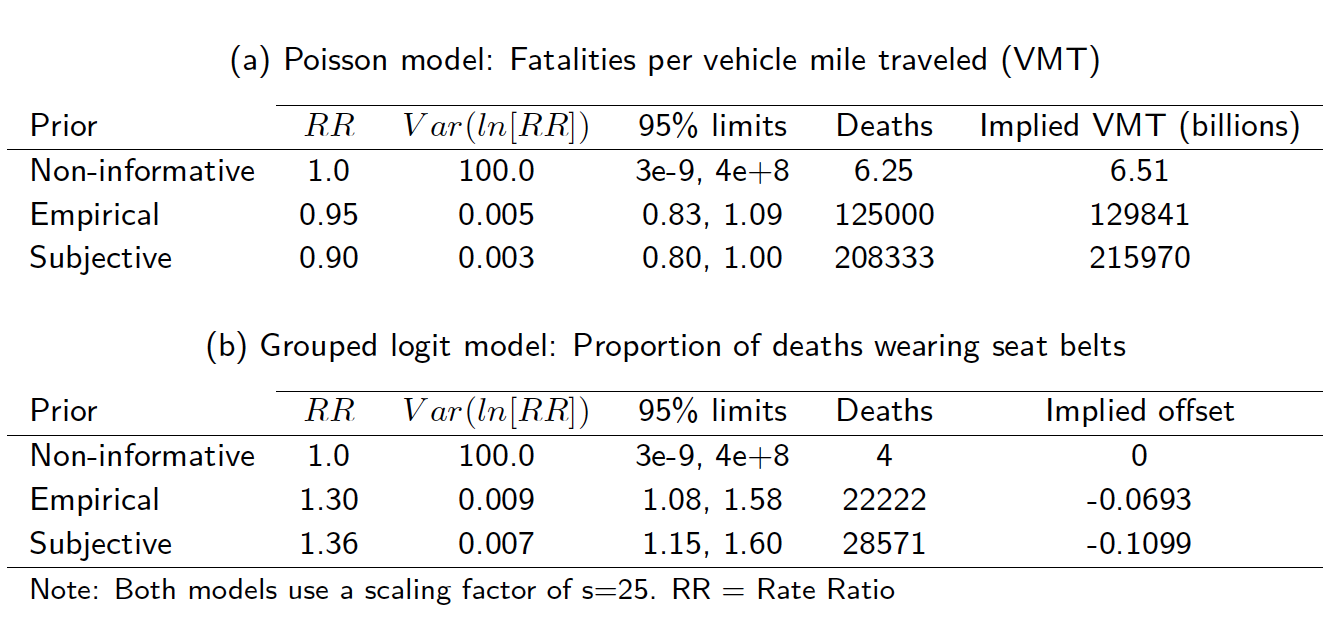
\includegraphics[width=0.95\paperwidth,bb = 0 0 200 100, draft, type=eps]{/Users/samharper/Dropbox/FARS/mvc-bayes/work/talk/t1rr.png}
\par\end{center}

\end{frame}
%
\begin{frame}{Data}
\begin{itemize}
\item Person-level data on fatal crashes and vehicle miles traveled (VMT)
from the Fatal Analysis Reporting System (FARS), 2000-2016.
\begin{itemize}
\item Aggregate to 10 ages, 50 states, 17 years (n=8500, $\sim$400k deaths).
\end{itemize}
\item Dates of primary enforcement upgrades from the Insurance Institute
for Highway Safety.\medskip{}
\item Other time-varying state policies:
\begin{itemize}
\item Speed limits;
\item Graduated driver's license programs;
\item Blood alcohol content laws.\medskip{}
\end{itemize}
\item Other time-varying state covariates:
\begin{itemize}
\item Police per capita;
\item Per capita alcohol consumption;
\item Median income.
\end{itemize}
\end{itemize}
\end{frame}
%
\begin{frame}[plain]{Study design: Difference-in-Differences}
\footnote{Meyer (1995); Angrist \& Pischke (2009); Ryan et al. (2015)}
\begin{itemize}
\item Use pre/post data on treated and control groups to estimate the effect
of policy.
\end{itemize}
\begin{center}
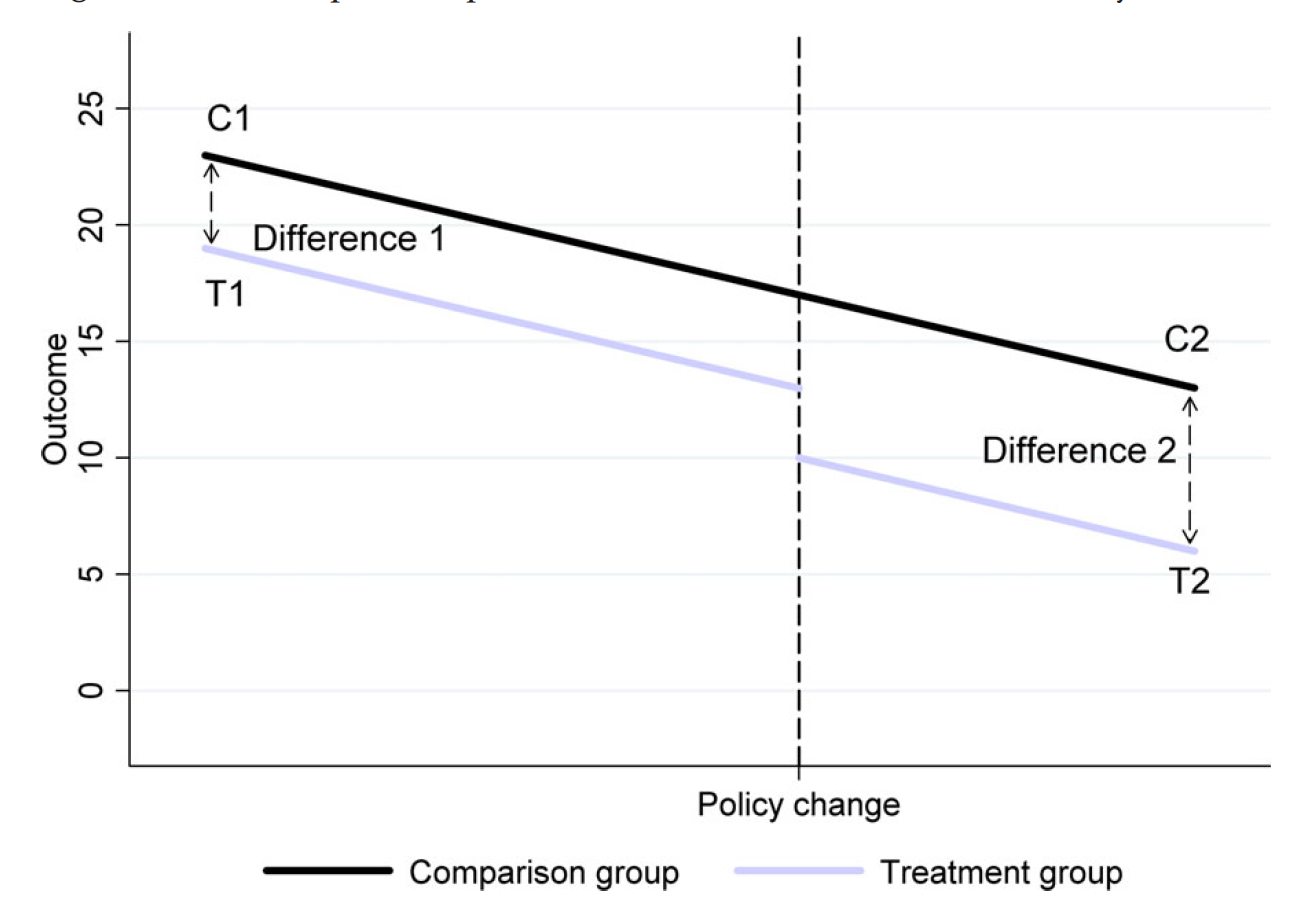
\includegraphics[width=0.9\textheight,bb = 0 0 200 100, draft, type=eps]{/Users/samharper/Dropbox/FARS/mvc-bayes/work/talk/ryan-fig1.png}
\par\end{center}

\end{frame}
%
\begin{frame}{Likelihood model specifications}
\begin{itemize}
\item For MVC death rates, Poisson model, i.e., $y_{ast}\sim Poisson(\mu_{ast})$:
\end{itemize}
\[
ln(\mu_{ast})=\alpha+{\color{red}\beta\times Primary_{st}}+\boldsymbol{\gamma}\mathbf{A}_{ast}+\boldsymbol{\delta}\mathbf{Z}_{st}+\boldsymbol{\sigma}_{s}+\boldsymbol{\tau}_{t}+ln\left(VMT_{ast}\right)
\]
\medskip{}

\begin{itemize}
\item For proportion belted, grouped logit model:
\end{itemize}
\[
ln\left(p_{ast}/[1-p_{ast}]\right)=\alpha+{\color{red}\beta\times Primary_{st}}+\boldsymbol{\gamma}\mathbf{A}_{ast}+\boldsymbol{\delta}\mathbf{Z}_{st}+\boldsymbol{\sigma}_{s}+\boldsymbol{\tau}_{t}
\]

\medskip{}

\begin{itemize}
\item {\small{}where ($Primary=1$ when a primary enforcement law is in
effect), and $\boldsymbol{\gamma}$, $\delta$, $\boldsymbol{\sigma}$,
and $\mathsf{\boldsymbol{\tau}}$ represent vectors of coefficients
for age groups, other time-varying state covariates{*}}\footnote{{\footnotesize{}{*}speed limit laws, graduated driver\textquoteright s
license laws, BAC laws, alcohol consumption per capita, police officers
per capita, state median income, police reported alcohol involved,
and proportion of crash deaths on rural roads.}}{\small{}, state fixed effects, and year fixed effects, respectively.}{\small \par}
\item {\small{}SEs clustered by state, marginal effects.}{\small \par}
\end{itemize}
\end{frame}
%

\section{Results}
\begin{frame}[plain]{Some descriptive comparisons}
\begin{center}
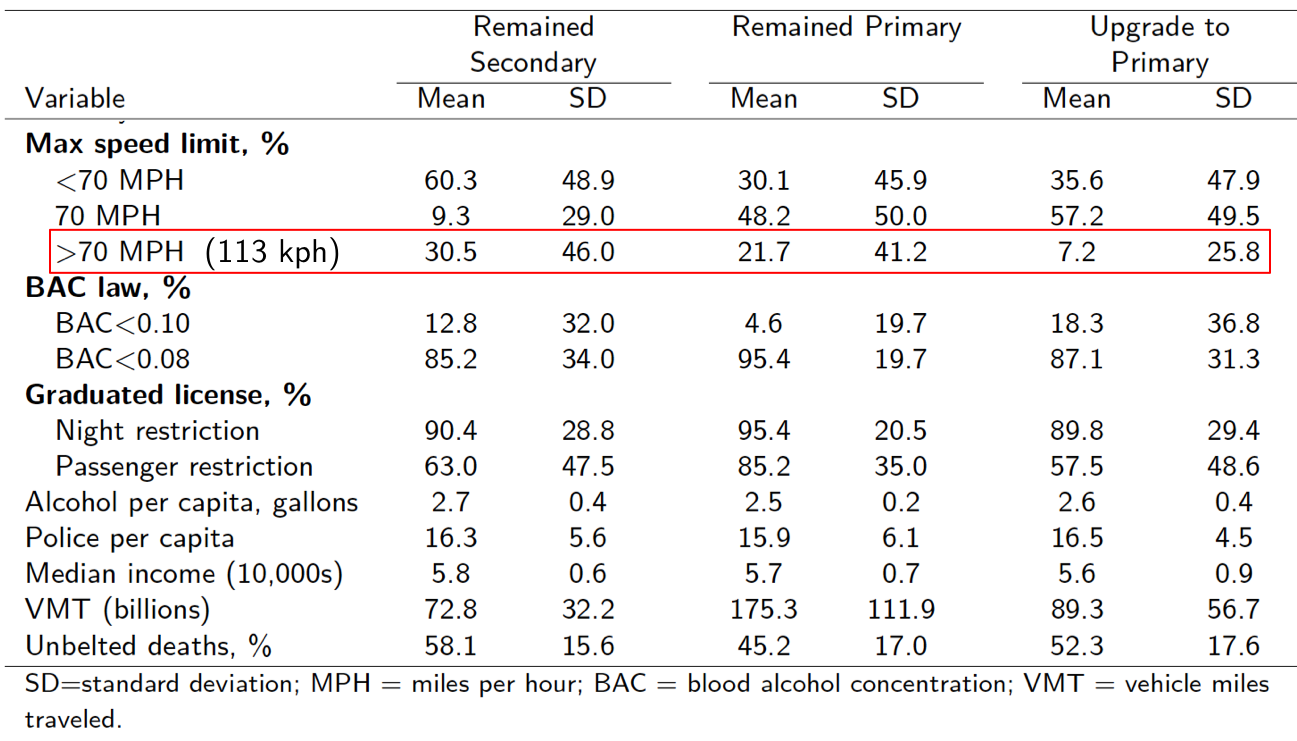
\includegraphics[width=0.9\paperwidth,bb = 0 0 200 100, draft, type=eps]{/Users/samharper/Dropbox/FARS/mvc-bayes/work/talk/t2.png}
\par\end{center}

\end{frame}
%
\begin{frame}[plain]{}
\begin{center}
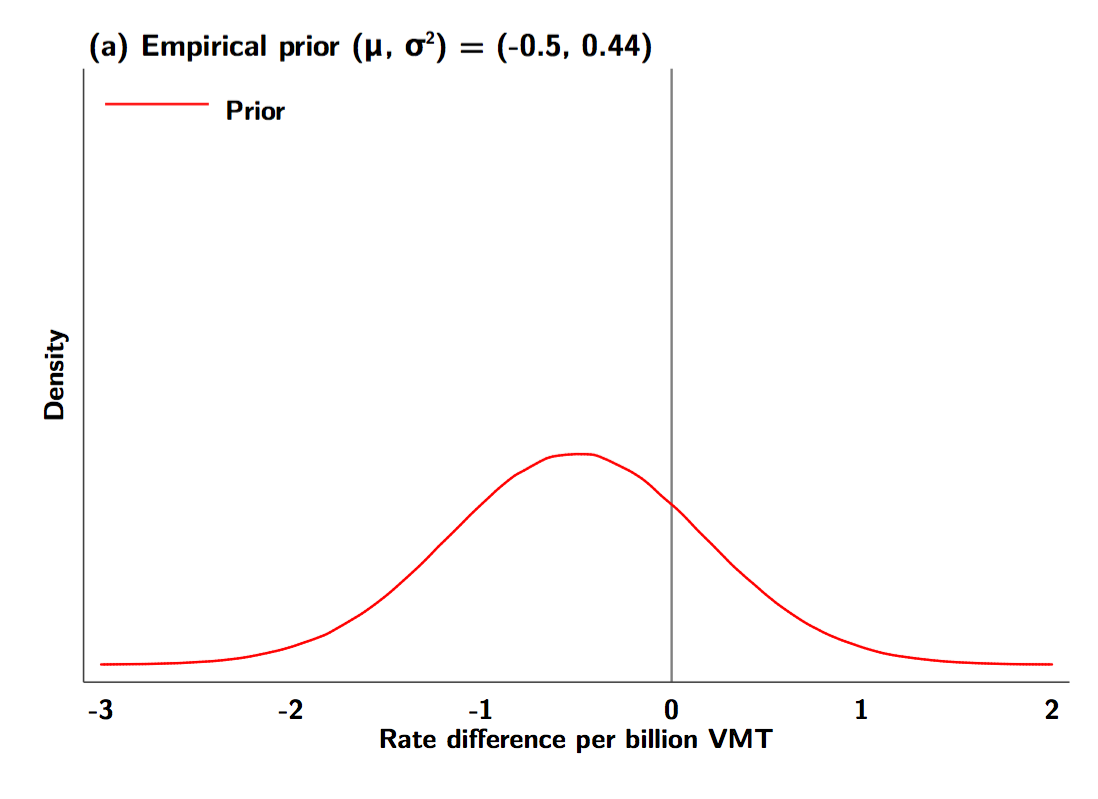
\includegraphics[width=0.95\paperwidth,bb = 0 0 200 100, draft, type=eps]{/Users/samharper/Dropbox/FARS/mvc-bayes/work/talk/prior2rd1.png}
\par\end{center}

\end{frame}
%
\begin{frame}[plain]{}
\begin{center}
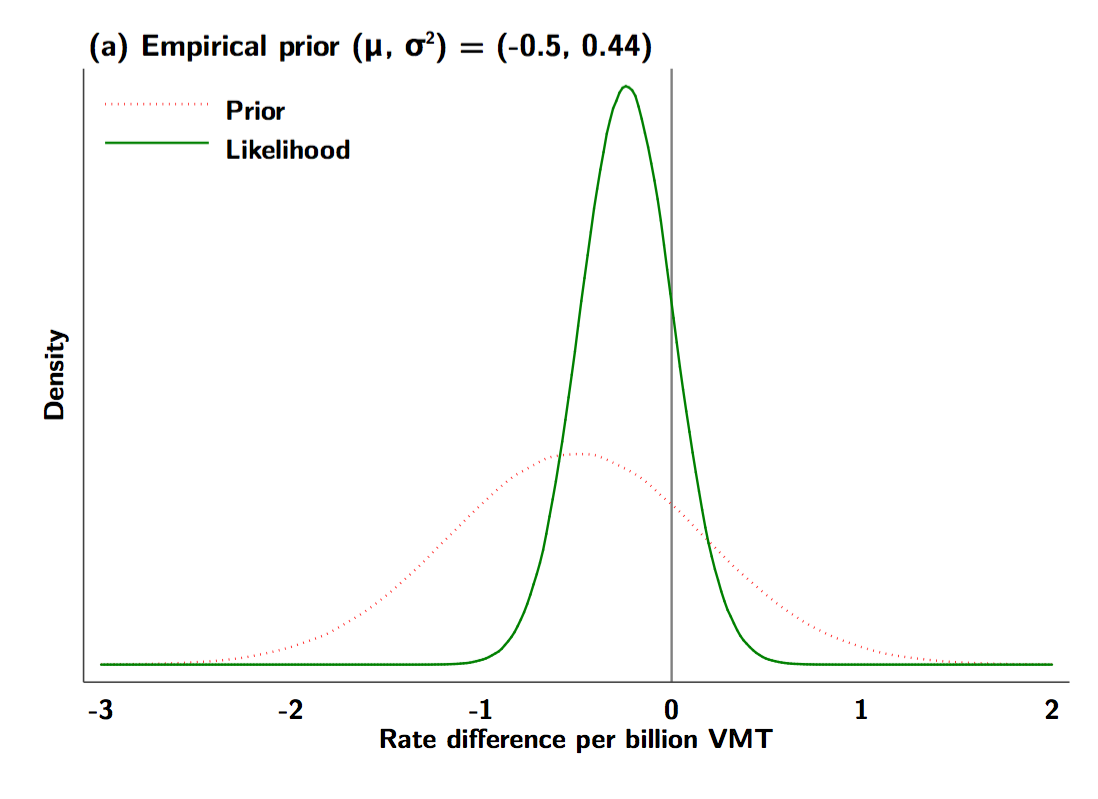
\includegraphics[width=0.95\paperwidth,bb = 0 0 200 100, draft, type=eps]{/Users/samharper/Dropbox/FARS/mvc-bayes/work/talk/prior2rd2.png}
\par\end{center}

\end{frame}
%
\begin{frame}[plain]{}
\begin{center}
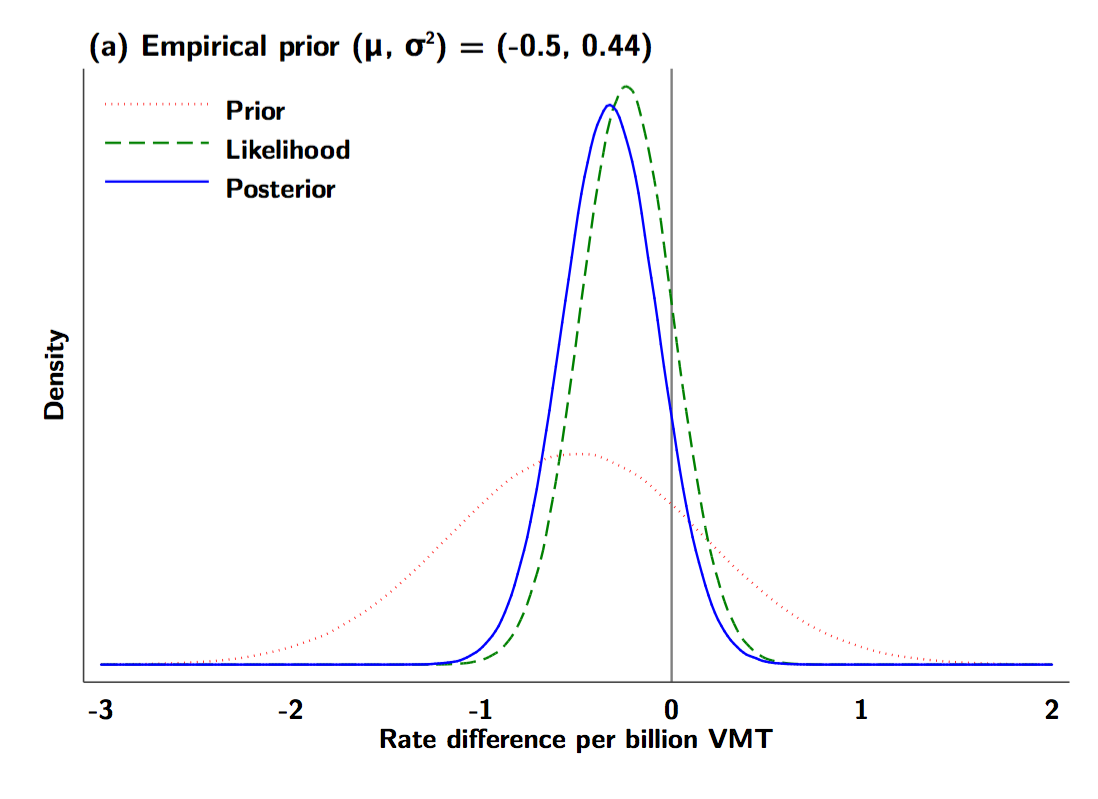
\includegraphics[width=0.95\paperwidth,bb = 0 0 200 100, draft, type=eps]{/Users/samharper/Dropbox/FARS/mvc-bayes/work/talk/prior2rd3.png}
\par\end{center}

\end{frame}
%
\begin{frame}[plain]{}
\begin{center}
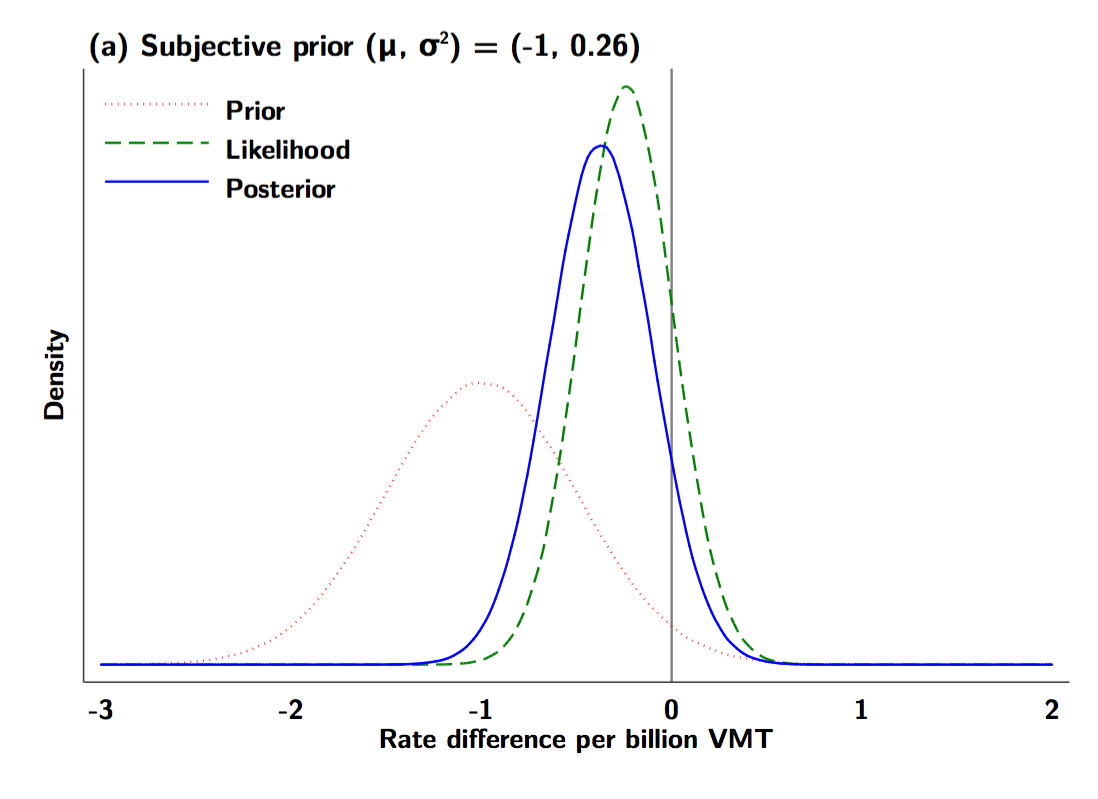
\includegraphics[width=0.95\paperwidth,bb = 0 0 200 100, draft, type=eps]{/Users/samharper/Dropbox/FARS/mvc-bayes/work/talk/prior3rd3.png}
\par\end{center}

\end{frame}
%
\begin{frame}[plain]{Results for MVC deaths}
\begin{center}
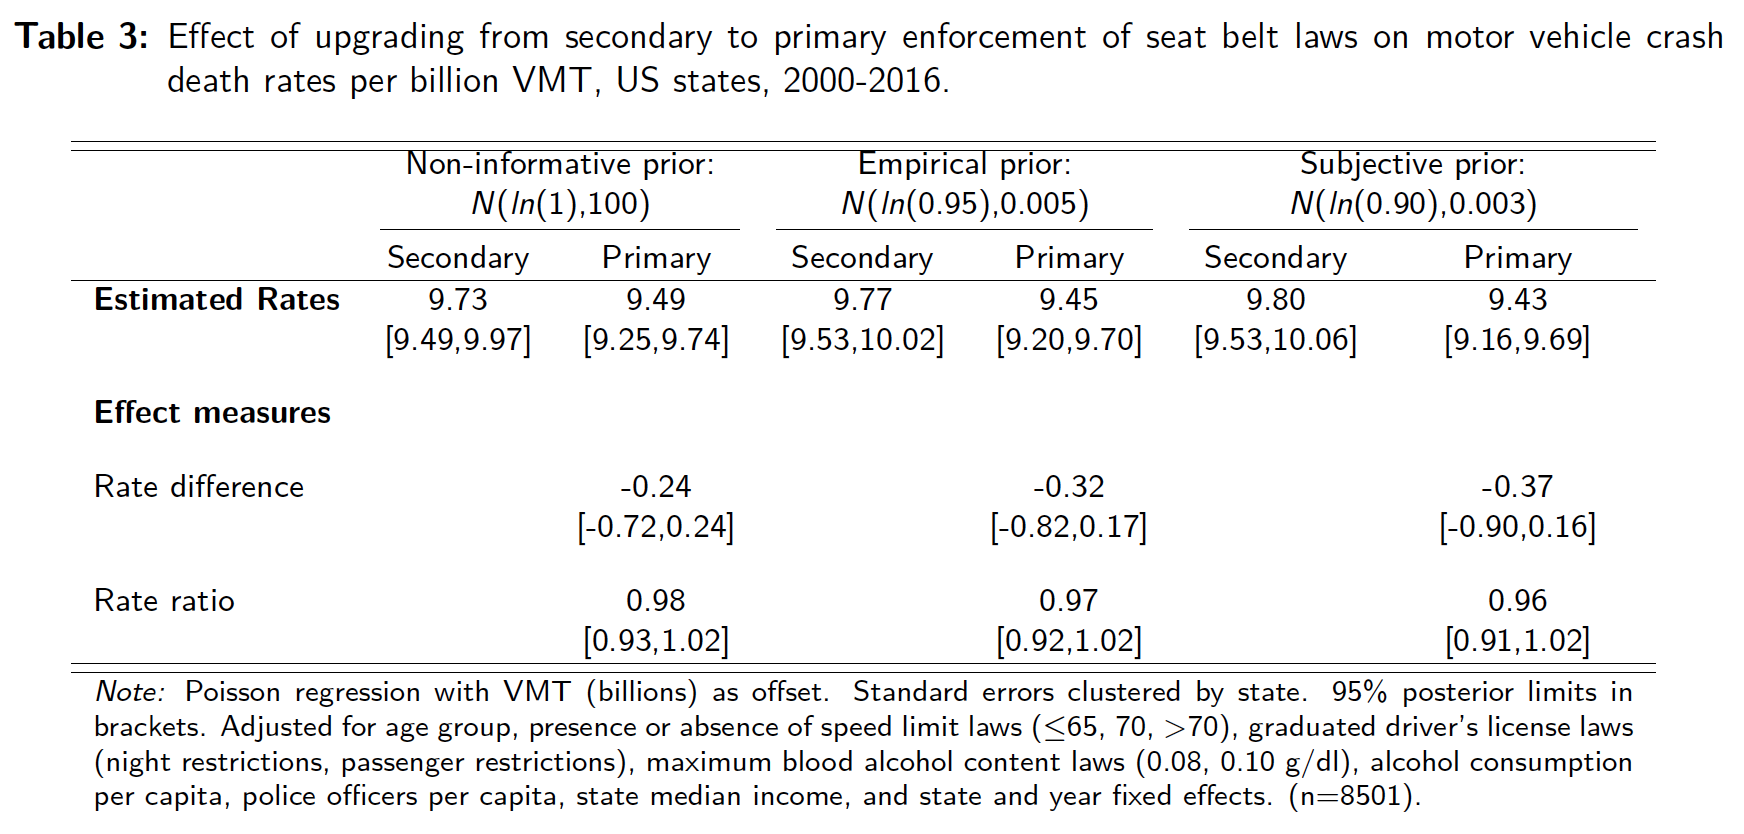
\includegraphics[width=0.95\paperwidth,bb = 0 0 200 100, draft, type=eps]{/Users/samharper/Dropbox/FARS/mvc-bayes/work/talk/t3.png}
\par\end{center}

\end{frame}
%
\begin{frame}[plain]{Results for proportion belted}
\begin{center}
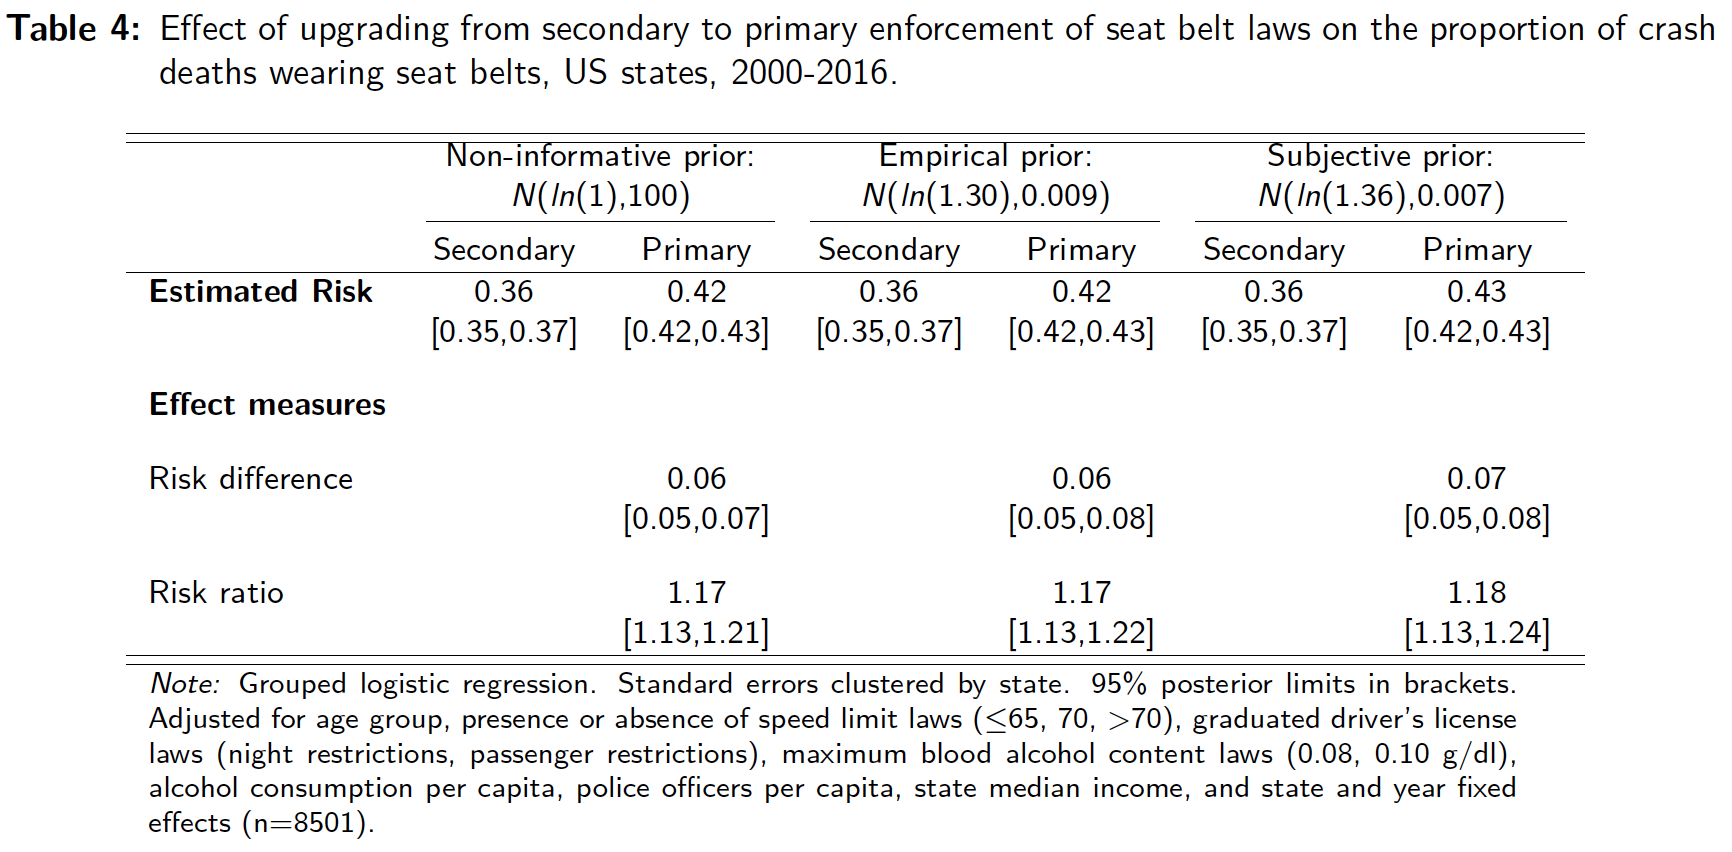
\includegraphics[width=0.95\paperwidth,bb = 0 0 200 100, draft, type=eps]{/Users/samharper/Dropbox/FARS/mvc-bayes/work/talk/t4.png}
\par\end{center}

\end{frame}
%
\begin{frame}[plain]{Sensitivity analysis with subjective priors}
\begin{center}
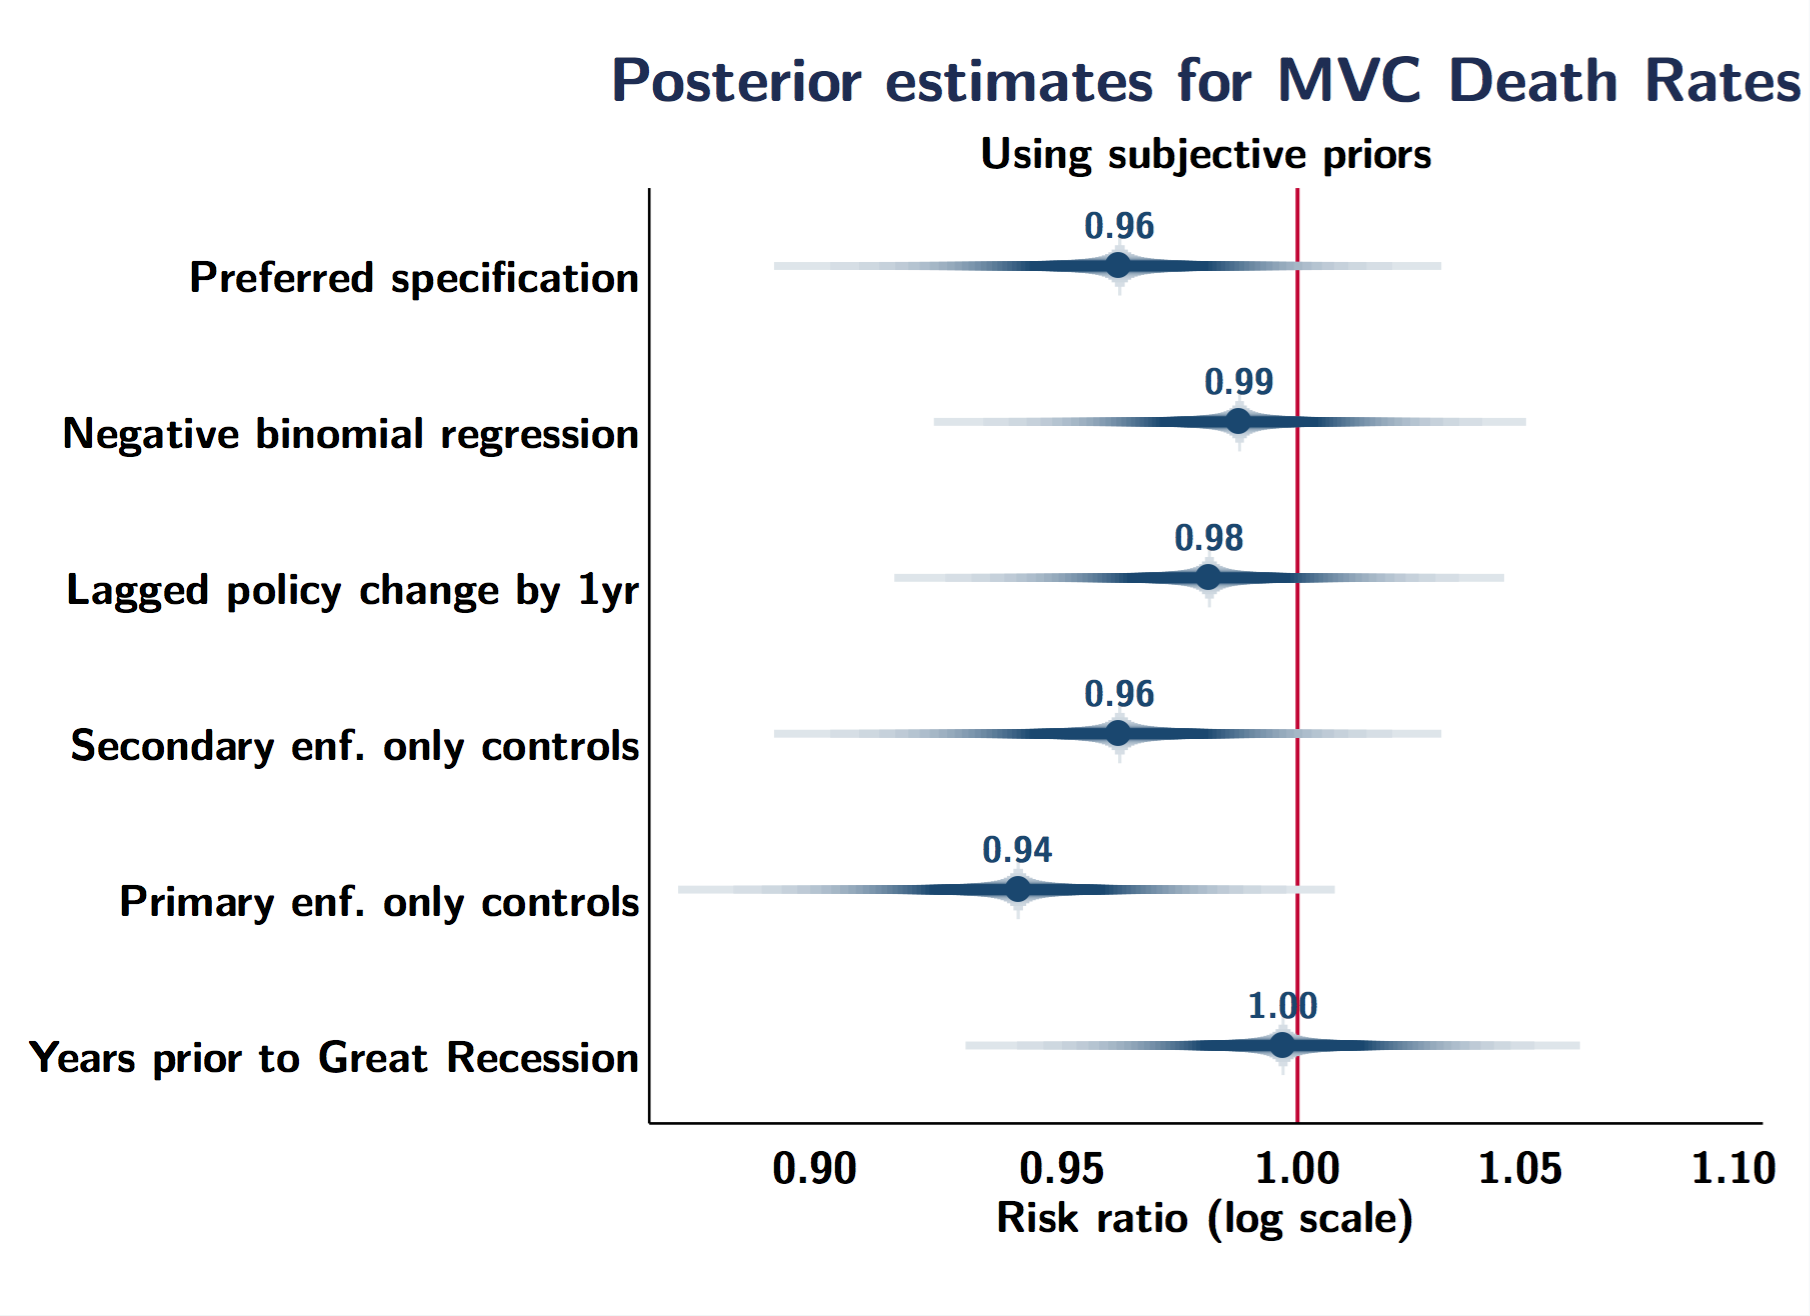
\includegraphics[width=0.9\paperwidth,bb = 0 0 200 100, draft, type=eps]{/Users/samharper/Dropbox/FARS/mvc-bayes/work/talk/rrplot-sens.png}
\par\end{center}

\end{frame}
%
\begin{frame}[plain]{Compare to fully Bayesian analysis}
\footnote{{*}Rstan model \texttt{bglm2} above, 4 chains, each with iter = 2000;
warmup = 1000; thin = 1; total post-warmup samples = 4000)}
\begin{itemize}
\item Consistent with fully Bayesian estimates
\item Clustered standard errors more challenging in full Bayes
\end{itemize}
\begin{center}
\begin{tabular}{lccc}
\hline 
 &
\multicolumn{3}{c}{Posterior estimates from Poisson}\tabularnewline
\cline{2-4} 
Model  &
Mean &
95\% LL &
95\% UL\tabularnewline
\hline 
\textit{Non-informative priors for all parameters} &
 &
 &
\tabularnewline
\enskip{}Semi-Bayes &
 -0.023 &
-0.073 &
0.027\tabularnewline
\enskip{}Full Bayes{*} &
-0.016 &
-0.029 &
-0.003\tabularnewline
\textit{$N(-1,0.05)$ for law, default for others} &
 &
 &
\tabularnewline
\enskip{}Semi-Bayes &
-0.037 &
-0.092 &
0.019\tabularnewline
\enskip{}Full Bayes{*} &
-0.034 &
-0.047 &
-0.021\tabularnewline
\hline 
\end{tabular}
\par\end{center}

\end{frame}
%

\section{Discussion}
\begin{frame}{Interpretation}
\begin{itemize}
\item Given our empirical priors, model, assumptions, and data, we can revise
our inference.\medskip{}
\item Impact on MVC deaths per billion VMT:
\begin{itemize}
\item We were 95\% certain true effect was in the interval (-1.7, 0.9)
\item Now we are 95\% certain the true effect is in the interval (-0.89,
0.35).
\end{itemize}
\medskip{}

\item<2-> Impact on proportion belted:
\begin{itemize}
\item We were 95\% certain true effect was in the interval (0.03, 0.23)
\item Now we are 95\% certain the true effect is in the interval (0.04,
0.07)
\end{itemize}
\medskip{}

\item<3-> For both outcomes, likelihood gets more weight, updated evidence
is toward the null. 
\end{itemize}
\end{frame}
%
\begin{frame}{Implications}
\begin{itemize}
\item MVC death rates still declining over this period.
\end{itemize}
\begin{center}
\includegraphics[height=0.8\textheight]{6_Users_samharper_Dropbox_work_research_projects_FARS_mvc-bayes_work_talk_fig1.png}
\par\end{center}

\end{frame}
%
\begin{frame}{Conclusions}
\begin{itemize}
\item Incorporating new evidence suggests weaker impact of primary laws
on death rates and proportion of deaths belted.\medskip{}
\item<2-> May imply other mechanisms contributing to declines in MVC death
rates
\begin{itemize}
\item Improved road and vehicle technology;
\item Traffic calming measures.\medskip{}
\end{itemize}
\item<3-> Possible that recent converts to seat belt use (due to law upgrades)
are a subpopulation with different risks.

\medskip{}

\item<4-> Incorporating prior evidence can help provide better estimates of
future policy impacts. 
\end{itemize}
\end{frame}
%
\begin{frame}{Reproducible materials}
\begin{itemize}
\item Code and data on my OSF page (https://osf.io/em2y7/)
\end{itemize}
\begin{center}
\includegraphics[height=0.8\textheight]{7_Users_samharper_Dropbox_work_research_projects_FARS_mvc-bayes_work_talk_osf-pic.png}
\par\end{center}

\end{frame}
%
\begin{frame}{Acknowledgements}

\begin{itemize}
\item No specific funding for this project.\medskip{}
\item Canadian Institutes for Health Research\medskip{}
\item Salary award from Fonds de recherche du Quebec \textendash{} Sante\medskip{}
\item Smarter Choices for Better Health Initiative, Erasmus University

\noindent {\large{}\bigskip{}
}{\large \par}
\end{itemize}
\noindent \begin{center}
{\large{}Thank you!}
\par\end{center}{\large \par}

\noindent \begin{center}
{\large{}sam.harper@mcgill.ca\qquad{}\includegraphics[scale=0.3]{8_Users_samharper_Dropbox_work_research_project____2018-10-visit_kickoff_kickoff-talk_twitter.png}@sbh4th}
\par\end{center}{\large \par}

\end{frame}
%

\end{document}
